\chapter{有限元离散化}
经过第二章和第三章的前期准备,本章开始我们正式开始讨论有限元离散化的问题。
\section{有限元离散的步骤}
\subsection{变分问题}
考虑抽象的变分问题:
\begin{definition}{变分问题}
    \label{def:variationProblem}
设$V$是某个无限维Banach空间,且$a(\cdot,\cdot)$和$f$分别为满足Lax-Milgram定理条件的双线性型和线性泛函,变分问题的描述为:求$u\in V$使得$\forall v\in V$,
\begin{equation}
    \label{eq:variationalProblem}
    a(u,v)=f(v).
\end{equation}
\end{definition}
根据第二章的Lax-Milgram定理,可知\ref{def:variationProblem}的解存在唯一。但$V$是一个无穷维空间,直接在$V$上求解弱形式依旧是一件无法完成的任务。

回想第一章我们对ode边值问题的讨论,我们选取了分段线性函数子空间$V_{h}\le V$,然后在这个有限维空间上求解了弱形式\eqref{eq:variationalProblem},并把$V_{h}$空间上的弱解作为$V$上弱解的一种近似。这种思路被称作\textbf{Galerkin方法}。同样的,对于一般情形下的问题,我们也可以定义与之相对应的\textbf{Galerkin方法}和\textbf{Ritz方法}。

假设$V_{h}\le V$是已经给定的有限维子空间,那么:
\begin{definition}{Galerkin}
    \textbf{Galerkin}方法的思路是求解$u_{h}\in V_{h}$,使得
    \begin{equation}
        \label{eq:GalerkinGeneral}
        a(u_{h},v_{h})=f(v_{h}).
    \end{equation}
\end{definition}
由Lax-Milgram定理,可知Galerkin方法求得的近似解也具有唯一性。

如果$a(u,v)$是一个对称双线性型,那么\eqref{eq:GalerkinGeneral}等价于一个最优化问题,\textbf{Ritz方法}就是着眼于求解这个最优化问题的思路。

\begin{definition}{Ritz}
    \textbf{Ritz}方法的思路是求解$u_{h}\in V_{h}$使得:
    \begin{equation}
        \label{eq:FunctionalMinimize}
        J(u_{h})=\min_{v_{h}\in V_{h}}J(v_{h}).
    \end{equation}
    其中
    \begin{equation}
        \label{eq:DefOfJ}
        J(v)=\frac{1}{2}a(v,v)-f(v).
    \end{equation}
\end{definition}

第二章我们已经证明过求解弱形式和优化问题的等价性。

一般的有限元离散问题,在给出Ritz方法和Galerkin方法的描述之后,就产生了下面两个主要的问题:
\begin{itemize}
    \item 如何确定子空间$V_{h}\le V$?
    \item 如何寻找子空间$V_{h}$的一组基使得问题容易求解?
\end{itemize}
本章将给出这两个问题的回答,并特别针对二维空间的问题,给出一整套可行的有限元计算方案。
\subsection{有限元子空间}
对于ode边值问题,我们用区间段的形式对整个区间$[0,1]$进行划分,对应的基函数即为数值分析课程中讲授的"hat-function"。在考虑高维区域时,继续使用分片多项式逼近依旧是一个好主意,但此时对区域$\Omega$的划分方案就不得不进行一些改变。

\begin{definition}{单形}
    一个$k-$单形是一个由$k+1$个顶点组成的$k-$维多面体凸包。设$x_{0},\cdots,x_{n}\in\mathbb{R}^{n}$且仿射无关,那么$n$维单形定义为:
    \begin{equation}
        \label{eq:nSimplex}
        K_{n}:=\left\{\sum_{i=0}^{n}\theta_{i}x_{i}:\sum_{i=0}^{n}\theta_{i}=1,\theta_{j}\ge0\forall j\in[0,n]\cap\mathbb{Z}\right\}.
    \end{equation}
\end{definition}
对于$\mathbb{R}^{n}$空间的有界区域$\Omega$,我们使用$n$-单形对其进行划分。假设我们对区域$\Omega$的单形剖分为$\mathscr{T}_{h}$,$T$为$\mathscr{T}_{h}$的\textbf{单元},那么我们对这样的单形剖分有下面这些要求:
\begin{enumerate}
    \item 对单元$T$的要求:
    \begin{itemize}
        \item $\forall T\in\mathscr{T}_{h}$,$T$为闭集,其内部$\mathring{T}$非空且连通。
        \item $\partial T$是Lipschitz-连续的。
        \item $\bar{\Omega}=\cup_{T\in\mathscr{T}_{h}} T$。
        \item 对于任何两个不同的$T_{1},T_{2}\in\mathscr{T}_{h}$,均有$\mathring{T_{1}}\cap\mathring{T_{2}}=\phi$。
        \item 对每个$T\in\mathscr{T}_{h}$,$\partial T$或者是$\partial\Omega$的一部分,或者是相邻单元$T'$的边。
    \end{itemize}
    \item 对于其上求解的多元分片多项式,$h\rightarrow 0$时,解收敛到原问题的解。
    \item 基函数的支集尽量小,使得计算简单。所得的刚度矩阵应当是稀疏矩阵。
\end{enumerate}
\begin{figure}[H]
    \begin{minipage}[t]{0.45\textwidth}
    \centering
    \caption{正确的单形剖分}
    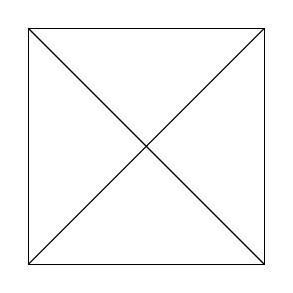
\begin{tikzpicture}
        \draw (0,0) rectangle (3,3);
        \draw (0,0)--(3,3);
        \draw (0,3)--(3,0);
    \end{tikzpicture}
    \end{minipage}
    \begin{minipage}[t]{0.45\textwidth}
    \centering
    \caption{错误的单形剖分}
    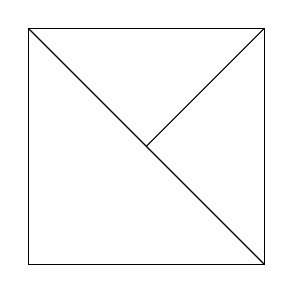
\begin{tikzpicture}
        \draw (0,0) rectangle (3,3);
        \draw (0,3)--(3,0);
        \draw (1.5,1.5)--(3,3);
    \end{tikzpicture}
    \end{minipage}
\end{figure}
有了空间划分$\mathscr{T}_{h}$后,定义在该划分空间上的分片多项式即可构成子空间$V_{h}\le V$。

\subsection{离散线性方程组与求解}
若$\dim(V_{h})=N$,设$\phi_{1},\phi_{2},\cdots,\phi_{N}$为$V_{h}$上的一组基函数,设
\begin{equation}
    u_{h}(x)=\sum_{i=1}^{N}u_{i}\phi_{i}(x),v_{h}(x)=\sum_{i=1}^{N}v_{i}\phi_{i}(x),
\end{equation}
代入\eqref{eq:GalerkinGeneral}, 我们有:
\begin{equation}
    \sum_{i=1}^{N}a(\phi_{i},\phi_{j})u_{i}=f(\phi_{j}),
\end{equation}
这是一个线性系统,求解该系统即可得到$u(x)$的近似值$u_{h}(x)$(事实上是一个分片多项式)。类似对ode边值问题的讨论,我们依旧可以称矩阵$K=(a(\phi_{i},\phi_{j}))_{ij}$为\textbf{刚度矩阵},$F=(f_{j})_{j=1}^{N}$为\textbf{负载向量}。

如果$a(\cdot,\cdot)$是对称的,Galerkin方法和Ritz方法等价。

对于刚度矩阵$K$,我们有下面的结论:
\begin{proposition}
    设$a(\cdot,\cdot):V\times V\rightarrow \mathbb{R}^{n}$是对称且V-椭圆的双线性形式,那么对应Galerkin-Ritz变分问题近似解的刚度矩阵$K$是对称正定的。
\end{proposition}
\begin{proof}
    对称性由$a(\cdot,\cdot)$的对称性可即刻得到。对于正定性,取$v\in\mathbb{R}^{n}$,记
    \begin{equation}
        v_{h}(x)=\sum_{i=1}^{N}v_{i}\phi_{i}(x),
    \end{equation}
    那么:
    \begin{equation}
        v^{t}Kv=a(v_{h},v_{h})\ge a\norm{v_{h}}^{2}\ge 0.
    \end{equation}
    该式取等号当且仅当$v_{h}=0$,即$v=0$。由此,矩阵$K$是正定的。
\end{proof}
\begin{remark}
    上面的性质保证了在变分问题的左侧项$a(\cdot,\cdot)$满足一定条件的情况下,其对应的离散化线性方程组的解存在唯一,且可以通过针对正定矩阵的算法进行求解。
\end{remark}
以上推导均需要满足\textbf{Lax-Milgram引理},因此需要$V_{h}$是$V$的子空间,这种有限元方法被称为\textbf{协调有限元方法}。

对于一个具体的问题,$V=H^{1}(\Omega)$,那么$V_{h}$中的分段多项式也必须在$H^{1}(\Omega)$中。这就要求我们对分段多项式在单元交界处的行为给出一些额外的条件。下面两个定理说明了分片多项式成为$V_{h}$中元素的充要条件。

\begin{theorem}
    设$v\in H^{1}(T),\forall T\in\mathscr{T}_{h}$,且$v\in C^{0}(\bar{\Omega})$,则$v\in H^{1}(\Omega)$。
\end{theorem}
\begin{proof}
    只需要证明$v$的广义导数$D_{i}v\in L^{2}(\Omega)$,即:
    \begin{equation}
        \label{eq:GeneralL2}
        -\int_{\Omega}D_{i}v\cdot\phi\dif x=\int_{\Omega}v\cdot\partial_{i}\phi\dif x,\forall\phi\in D(\Omega).
    \end{equation}
由于$v\in C^{0}(\bar\Omega)$,且$v$在每个单元$T$上均为多元多项式,在每个单元$T$上运用Gauss-Green公式,有:
\begin{equation}
    \label{eq:GaussGreen4GL2}
    \int_{\Omega}v\cdot\partial_{i}\phi\dif x=\sum_{T\in\mathscr{T}_{h}}\int_{T}v\cdot\partial_{i}\phi\dif x=-\sum_{T}\int_{T}D_{i}v\cdot\phi\dif x+\sum_{T}\int_{\partial T}v\phi\cdot n_{i}\dif s.
\end{equation}
$n_{i}$表示单位法向量在第$i$个维度下的投影。由\eqref{eq:GaussGreen4GL2},要证\eqref{eq:GeneralL2},即证
\begin{equation}
    \label{eq:BoundaryCond}
    \sum_{T}\int_{\partial T}v\phi\cdot n_{i}\dif s=0.
\end{equation}
根据我们选取单元$T$的第五点要求,取$T_{0}\in\partial T$,有两种情况:
\begin{itemize}
    \item $T_{0}$是区域$\Omega$的边界:由$\phi\in D(\Omega)$,即$\phi|_{\partial\Omega}=0$,可知$\int_{T_{0}}v\phi\cdot n_{i}\dif s=0$。
    \item $T_{0}$是两个单元$T_{a}$和$T_{b}$的交线。此时积分式\eqref{eq:BoundaryCond}中有关线段$T_{0}$的积分表达式为
    \begin{equation}
        \label{eq:EliminateEdge}
        \int_{T_{0}\in T_{a}}v\phi\cdot n_{i}\dif s+\int_{T_{0}\in T_{b}}v\phi\cdot n_{i}\dif s.
    \end{equation}
\end{itemize}
    由于在$T_{a}$和$T_{b}$上,线段$T_{0}$位置相同,法向量方向相反,从而\eqref{eq:EliminateEdge}的值为0。故\eqref{eq:BoundaryCond}得证,即\eqref{eq:GeneralL2}成立。
\end{proof}
\begin{theorem}
    设$v|_{T}\in C^{0}(T),\forall T\in\mathscr{T}_{h}$,且$v\in H^{1}(\Omega)$,则$v\in C^{0}(\bar{\Omega})$。
\end{theorem}
\begin{proof}
    如果$v$在两个相邻单元$e$和$e'$上不连续,即在其公共边$\gamma$上$v|_{e}-v|_{e'}$不恒为0。无妨其在$\gamma$上的某段处为正,作开集$U$使得$U\subset e\cap e'$,且$v|_{e}-v|_{e'}>0$在$U\cap\gamma$上成立,则作函数$\phi\in D(U)$使得在supp$(\phi)$上$\phi>0$。如果$v\in H^{1}(\Omega)$,根据$H^{1}(\Omega)$广义函数的定义,必定有:
    \begin{equation}
        \int_{U\cap\gamma}(v|_{e}-v|_{e'})\cdot\phi\cdot n_{i}^{e}\dif s=0.
    \end{equation}
    这与前面的假定相矛盾。
\end{proof}
\begin{remark}
    上面两个定理要求:我们求得的有限元逼近解必须在整个区域内是连续的。
\end{remark}
\section{二维情形}
在本节中,我们着眼于$\Omega\subset\mathbb{R}^{2}$,讨论区域$\Omega$的三角划分,以及定义在该划分上的分片多项式函数。

首先,我们讨论\textbf{定义在三角形有界区域上的}多项式函数。
\subsection{重心坐标}
一个很容易想到的思路是,依据三角形上某些点(例如三个顶点)处的函数取值,插值得到一个多元多项式。但如果采用直角坐标,插值多项式的表达式不免会显得非常麻烦。如果能通过一些合理的坐标变换,将一般三角形区域转化为等腰直角三角形区域,则可以大大降低该区域上插值多项式形式的复杂性。这就是引入\textbf{重心坐标}的原因。
\begin{figure}[H]
    \caption{重心坐标变换}
        \centering
        \begin{tikzpicture}
            \draw (0,0)--(1,3);
            \draw (1,3)--(2,2);
            \draw (2,2)--(0,0);
            \draw [->] (3,1.5)--(8,1.5);
            \draw (9,0)--(12,0);
            \draw (12,0)--(9,3);
            \draw (9,3)--(9,0);
        \end{tikzpicture}
\end{figure}
\begin{definition}{重心坐标}
    考虑平面上的三角形$\triangle A_{1}A_{2}A_{3}$,顶点编号为逆时针,设点$P(x,y)$落在三角形内部,则定义点$P$的\textbf{重心坐标}$(\lambda_{1},\lambda_{2},\lambda_{3})$为:
    \begin{equation}
        \lambda_{1}=\frac{m(\triangle PA_{2}A_{3})}{m(\triangle A_{1}A_{2}A_{3})},\lambda_{2}=\frac{m(\triangle PA_{1}A_{3})}{m(\triangle A_{1}A_{2}A_{3})},\lambda_{3}=\frac{m(\triangle PA_{1}A_{2})}{m(\triangle A_{1}A_{2}A_{3})}.
    \end{equation}
    其中$m$表示区域的测度,在这里表示的是三角形的面积。
\end{definition}
根据定义,下面的表达式是显然的:
\begin{equation}
    \label{eq:burycenterCoordProp}
    \lambda_{i}(A_{j})=\delta_{ij}.
\end{equation}
所以,定义在$\triangle A_{1}A_{2}A_{3}$的线性函数$u$可以表示为:
\begin{equation}
    u(x,y)=u(A_{1})\lambda_{1}(x,y)+u(A_{2})\lambda_{2}(x,y)+u(A_{3})\lambda_{3}(x,y).
\end{equation}
分别取$u(x,y)=x$,$u(x,y)=y$,$u(x,y)=1$,代入上式,可得下面的性质:
\begin{proposition}{直角坐标与重心坐标的关系}
   记$A_{i}$的坐标为$(x_{i},y_{i})$,$\triangle A_{1}A_{2}A_{3}$上直角坐标和重心坐标的关系式如下:
   \begin{equation}
    \left\{
        \begin{aligned}
            x&=x_{1}\lambda_{1}+x_{2}\lambda_{2}+x_{3}\lambda_{3}\\
            y&=y_{1}\lambda_{1}+y_{2}\lambda_{2}+y_{3}\lambda_{3}\\
            1&=\lambda_{1}+\lambda_{2}+\lambda_{3}.\\
        \end{aligned}
    \right.
   \end{equation} 
\end{proposition}
重心坐标有许多非常棒的性质,可以大大简化三角形区域上的函数计算。
\begin{proposition}{重心坐标的性质}
    \begin{enumerate}
        \item 三角形三顶点$A_{1},A_{2},A_{3}$,重心$G$的坐标分别为:
        \begin{equation}
            A_{1}(1,0,0), A_{2}(0,1,0), A_{3}(0,0,1), G(\frac{1}{3},\frac{1}{3},\frac{1}{3}).
        \end{equation}
        \item 三角形三边的方程:
        \begin{equation}
            A_{1}A_{2}:\lambda_{3}=0; A_{2}A_{3}:\lambda_{1}=0; A_{3}A_{1}:\lambda_{2}=0.
        \end{equation}
        \item 平行于三角形某一边(如$A_{1}A_{2}$)的方程:$\lambda_{3}=c$。
        \item 任一$x,y$的$k$次多项式是$\lambda_{1},\lambda_{2},\lambda_{3}$的$k$次齐次多项式,反之亦然。
        \item 由$\lambda_{1}+\lambda_{2}+\lambda_{3}=1$知这三个变量线性相关。如果取独立变量$\lambda_{1},\lambda_{2}$,则:
        \begin{equation}
            \left\{
                \begin{aligned}
                    \pdfFrac{}{\lambda_{1}}&=(x_{1}-x_3)\pdfFrac{}{x}+(y_1-y_3)\pdfFrac{}{y},\\
                    \pdfFrac{}{\lambda_{2}}&=(x_{2}-x_3)\pdfFrac{}{x}+(y_2-y_3)\pdfFrac{}{y}.\\
                \end{aligned}
            \right.
        \end{equation}
        \item 重心坐标和直角坐标变换的Jacobi行列式为:
        \begin{equation}
            \det\left(\pdfFrac{(x,y)}{(\lambda_{1},\lambda_{2})}\right)=2m(\triangle_{e}).
        \end{equation}
        $m(\triangle_{e})$为三角形单元的面积。
        \end{enumerate}
\end{proposition}
\begin{exercise}
    证明重心坐标的上述性质。
\end{exercise}
重心坐标对简化单元上的积分计算具有重要的价值,由于重心坐标把一般的三角形映射到直角边长为1的等腰直角三角形,我们可以把一般积分区域上的求积分问题转化为三角形区域上求积分的问题。记$e$为三角单元,$\hat{e}$为变换后的等腰直角三角形,具体推导如下:
\begin{equation}
    \label{eq:changevariables}
    \begin{aligned}
        \int\int_{e}F(x,y)\dif x\dif y&=\int\int_{\hat{e}}F(\lambda_{1},\lambda_{2})\det\pdfFrac{(x,y)}{(\lambda_{1}\lambda_{2})}\dif\lambda_{1}\dif\lambda_{2}\\
        &=2m(\triangle_{e})\int_{0}^{1}\dif\lambda_{1}\int_{0}^{1-\lambda_{1}}F(\lambda_{1},\lambda_{2},1-\lambda_{1}-\lambda_2)\dif\lambda_{2}.
    \end{aligned}
\end{equation}
下面的积分等式在有限元计算中是重要的:
\begin{proposition}
    \begin{equation}
        \label{eq:monomial}
        \int\int_{e}\lambda_{1}^{m}\lambda_{2}^{n}\lambda_{3}^{k}\dif x\dif y=2m(\triangle_{e})\frac{m!n!k!}{(m+n+k+2)!}.
    \end{equation}
\end{proposition}
\begin{exercise}
    证明\eqref{eq:monomial}。
\end{exercise}
以分片线性多项式元为例,在实际计算中,插值基函数选取为:在其中一个顶点取值为1,其余顶点取值均为0的分片线性函数。其形式与一维情形的hat-function比较类似,示意图如下:
\begin{figure}[H]
    \caption{二维分片线性插值基函数}
    \centering
    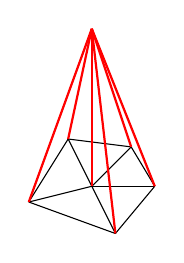
\begin{tikzpicture}
        \draw (0,0)--(0.5,0.5);
        \draw (0,0)--(0.8,0);
        \draw (0,0)--(0.3,-0.6);
        \draw (0,0)--(-0.3,0.6);
        \draw (0,0)--(-0.8,-0.2);
        \draw (0.5,0.5)--(0.8,0);
        \draw (0.8,0)--(0.3,-0.6);
        \draw (0.3,-0.6)--(-0.8,-0.2);
        \draw (-0.8,-0.2)--(-0.3,0.6);
        \draw (-0.3,0.6)--(0.5,0.5);
        \draw[color=red,thick] (0,0)--(0,2);
        \draw[color=red,thick] (0,2)--(0.5,0.5);
        \draw[color=red,thick] (0,2)--(0.8,0);
        \draw[color=red,thick] (0,2)--(0.3,-0.6);
        \draw[color=red,thick] (0,2)--(-0.3,0.6);
        \draw[color=red,thick] (0,2)--(-0.8,-0.2);
    \end{tikzpicture}
\end{figure}
\subsection{三角单元内分段多项式的形式}
本节中,我们借助重心坐标,在有合适插值条件的前提下,写出每个三角单元内部分片多项式的表达式。

如无特殊说明,本节中单元$e$指的是三角形$\triangle A_{1}A_{2}A_{3}$。
\subsubsection{线性Lagrange元}
二元线性多项式的自由度为3。要在单元$e$上确认一个线性二元多项式,需要三个插值条件,考虑在单元$e$的三个顶点处给出:
\begin{equation}
    \label{eq:LinearCond}
    u(A_{i})=u_{i},i=1,2,3.
\end{equation}
由重心坐标的性质,即
\begin{equation}
    \lambda_{i}(A_{j})=\delta_{ij},
\end{equation}
可得:
\begin{equation}
    p(x,y)=\sum_{i=1}^{3}u_{i}\lambda_{i}(x,y).
\end{equation}
这就是重心坐标下\textbf{线性Lagrange元}的表达式。
\subsubsection{完全二次Lagrange元}
$e$上的完全二次多项式可以表示为:
\begin{equation}
    p(x,y)=a_{0,0}+a_{1,0}x+a_{2,0}x^2+a_{0,1}y+a_{1,1}xy+a_{0,2}y^{2}.
\end{equation}
由表达式知共有6个自由变量,需要6个插值条件。在实际计算中,我们取三角形三个顶点以及三条边的中点作为插值节点,问题转化为求一组基函数使得$u_{i}(A_{j})=\delta_{ij}$。

插值节点如图所示:
\begin{figure}[H]
    \caption{插值节点示意,此处待完善,问题在于如何进行符号标注}
    \centering
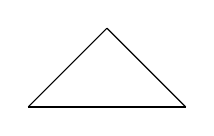
\begin{tikzpicture}
    \draw (0,0)--(2,0);
    \draw (2,0)--(1,1);
    \draw (1,1)--(0,0);
\end{tikzpicture}
\end{figure}
首先考虑构造二次多项式$p(\lambda_{1},\lambda_{2},\lambda_{3})$,使得在顶点$A_{1}$上的取值为1,在其他顶点和线段中点处取值均为0。由于$\lambda_{1}(A_{1})=1,\lambda_{1}(A_{i})=0(i\neq 1)$,可以取$\lambda_{1}$为$p$的一个因子。由于$A_{5}A_{6}$平行于$A_{2}A_{3}$,且为中点连线,故该线段的表达式为$\lambda_{1}=\frac{1}{2}$。从而$(2\lambda_{1}-1)$也是$p$的因子。此时取基函数$p(\lambda_{1},\lambda_{2},\lambda_{3})=\lambda_{1}(2\lambda_{1}-1)$,经检验可知该多项式在$A_{1}$取1,在$A_{i}(i\neq 1)$均取0。

下面考虑如何选取多项式使得中点处取值为1,其余为0。以$A_{1}A_{2}$的中点为例,在该点处,$\lambda_{1}=\lambda_{2}=\frac{1}{2},\lambda_{3}=0$。故一个比较合理的取法是$p(x,y)=4\lambda_{1}\lambda_{2}$。经验证知,该多项式满足基函数的要求。

因此,完全二次Lagrange元的表达式可以写为:
\begin{equation}
    p_{2}(x,y)=u_{1}\lambda_{1}(2\lambda_{1}-1)+u_{2}\lambda_{2}(2\lambda_{2}-1)+u_{3}\lambda_{3}(2\lambda_{3}-1)+4u_{6}\lambda_{1}\lambda_{2}+4u_{4}\lambda_{2}\lambda_{3}+4u_{5}\lambda_{3}\lambda_{1}.
\end{equation}
\subsubsection{完全三次Lagrange元}
完全三次Lagrange元需要10个插值节点,这里取三角形三个顶点,三条边上的三等分点以及三角形的重心。类似完全二次Lagrange元的讨论,完全三次Lagrange元的表达式可以写成:
\begin{equation}
    \label{eq:complete3order}
    p(x,y)=\sum_{i=1}^{3}u_{i}\frac{\lambda_{i}(3\lambda_{i}-1)(3\lambda_{i}-2)}{2}+\sum_{i\neq j}\frac{9}{2}\lambda_{i}\lambda_{j}(3\lambda_{i}-1)u_{iij}+27\lambda_{1}\lambda_{2}\lambda_{3}u_{123}.
\end{equation}
\begin{exercise}
    证明\eqref{eq:complete3order}中选取的函数确实构成一组插值基底。
\end{exercise}